In Versuch 245 befassen wir uns mit der elektromagnetischen Induktion. Diese beschreibt die Erzeugung von elektrischer Spannung durch zeitlich veränderlich Magnetfelder. Kern des Versuchs bildet das Induktionsgesetz, wessen Zusammensetzung wir in den einzelnen Versuchsteilen untersuchen werden. Das hierfür nötige Magnetfeld wird mit einer sogenannten Helmholtz-Spule erzeugt. Als Induktionsspule wird eine kleinere Spule im Inneren der Helmholtz-Spule verwendet, welche sich mit einem Motor in Rotation versetzen lässt.

\subsection{Physikalische Grundlagen}

\subsubsection{Induktionsgesetz}
Wird ein elektrischer Leiter einem zeitlich veränderlichen Magnetfeld ausgesetzt, so entsteht entlang diesem eine elektrische Spannung, die Induktionsspannung. Nach dem Induktionsgesetz
\begin{align}
  U_i(t) = - \dv{\Phi}{t}
\end{align}
entspricht die Induktionsspannung $U_i$ dem Negativen der zeitlichen Ableitung des magnetischen Flusses $\Phi$. Der magnetische Fluss wiederum ist definiert durch das Integral 
\begin{align}
  \Phi(t) = \int_{\va{A}(t)} \va{B}(t) \cdot \dd{\va{A}}
\end{align}
der (zeitabhängigen) magnetischen Flussdichte $\va{B}$ über eine (zeitabhängige) Fläche $\va{A}$.

Für den Spezialfall einer mit Kreisfrequenz $\omega$ rotierenden Flachspule mit Fläche $A$ und Windungszahl $N$ in einem konstanten Magnetfeld $B$ gilt für den magnetischen Fluss
\begin{gather}
  \Phi(t) = B A N \cos(\omega t)
  \intertext{und somit für die Induktionsspannung}
  U_{i}(t) = - B A N \omega \sin(\omega t).
\end{gather}

Hält man die Induktionsspule bei einem konstanten Winkel $\alpha$ und setzt diese dem Feld einer weiteren Spule aus, durch welche ein Wechselstrom der Kreisfrequenz $\Omega$ fließt, so ergibt sich die Induktionsspannung
\begin{align}
  U_i(t) = - BAN\Omega \sin(\Omega t) \cos(\alpha). \label{eq:ui_ac_angle}
\end{align}
Lässt man zusätzlich eine zeitliche Veränderung von $\alpha$ zu, versetzt also die Induktionsspule in Rotation, so zeigt sich für eine konstruktive Interferenz der Frequenzen eine Schwebung im Verlauf der induzierten Spannung.

\subsubsection{Selbstinduktion und Induktivität}
Die im vorherigen Absatz dargestellte zeitliche Änderung der Spannung in der felderzeugenden Spule führt dazu, dass in dieser Spule selbst eine Induktionsspannung entsteht. Diese erzeugte Spannung ist der angelegten Spannung entgegengerichtet. Die daher rührende Schwächung des Stroms durch die Spule lässt sich durch den induktiven Widerstand
\begin{align}
  X_L = \omega L \label{eq:indukt_widerst}
\end{align}
beschreiben. Die hierbei auftretende Konstante $L$ heißt \textit{Induktivität}. Jeder Art von Leiteranordnung lässt sich eine solche bestimmte Induktivität zuordnen. Hierbei spielt sie unter anderem bei der Bestimmung komplexer Impedanzen von Wechselstromkreisen eine Rolle.

\subsubsection{Helmholtz-Spule}
Die parallele Anordnung zweier in Reihe geschalteten Magnetspulen mit Radius $R$ im Abstand $R$ nennt man Helmholtz-Spule (siehe Abbildung \ref{fig:helmholtz_coil}).

Die Besonderheit dieser ist die Erzeugung eines homogenen Magnetfeldes im Zentrum der Spulenanordnung mit der Flussdichte
\begin{align}
  \va{B}(0) = \frac{8}{\sqrt{125}} \frac{\mu_0 N I}{R} \va{e}_x. \label{eq:b_hh}
\end{align}

An anderen Punkte der Symmetrieachse $x$ ist die magnetische Flussdichte im Allgemeinen nicht analytisch berechenbar.

\begin{figure}[H]
  \centering
  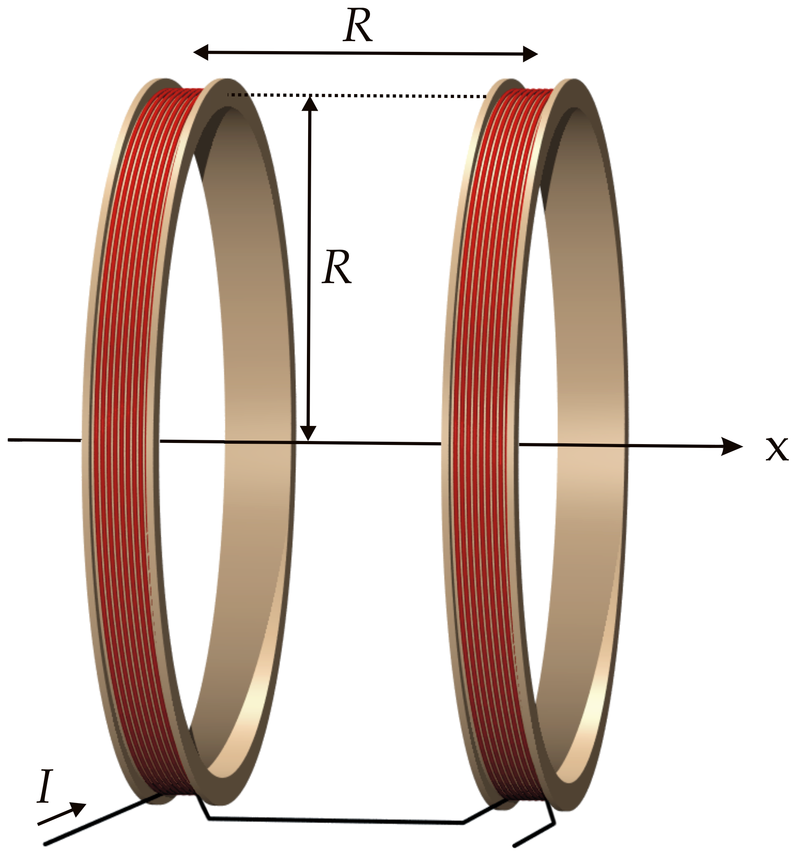
\includegraphics[width=0.5\textwidth]{files/Helmholtz_coils.png}
  \caption{Helmholtz-Spule}
  \label{fig:helmholtz_coil}
\end{figure}

Auch einer Helmholtz-Spule lässt sich eine Induktivität zuordnen.
\newpage\noindent
\subsubsection{Das Magnetfeld der Erde}

Durch die Bewegung von flüssigem Eisen im äußeren Erdkern wird ein Magnetfeld erzeugt. In erster Näherung lässt sich dieses Feld wie das Dipolfeld eines riesigen Stabmagneten im Zentrum der Erde beschreiben. Hierbei sind der magnetische Süd- und Nordpol ungefähr umgekehrt in Richtung des geografischen Nord- und Südpol ausgerichtet.

 Die \textit{Inklination} ist der Winkel, den die Feldlinien des Magnetfeldes relativ zur Horizontalen bilden. Wie in der schematischen Darstellung in Abbildung \ref{fig:erdmagnetfeld} zu sehen, verlaufen die Magnetfeldlinien am Äquator parallel zur Erdoberfläche, entsprechend einer Inklination von 0°, und an den Polen senkrecht zu dieser, entsprechend einer Inklination von 90°. Die Inklination in den Bereichen zwischen diesen lässt sich durch die Zerlegung des Erdmagnetfeldes in eine Horizontal- und eine Vertikalkomponente, mithilfe einer Kompensationsmessung, empirisch bestimmen.

\begin{figure}[H]
  \centering
  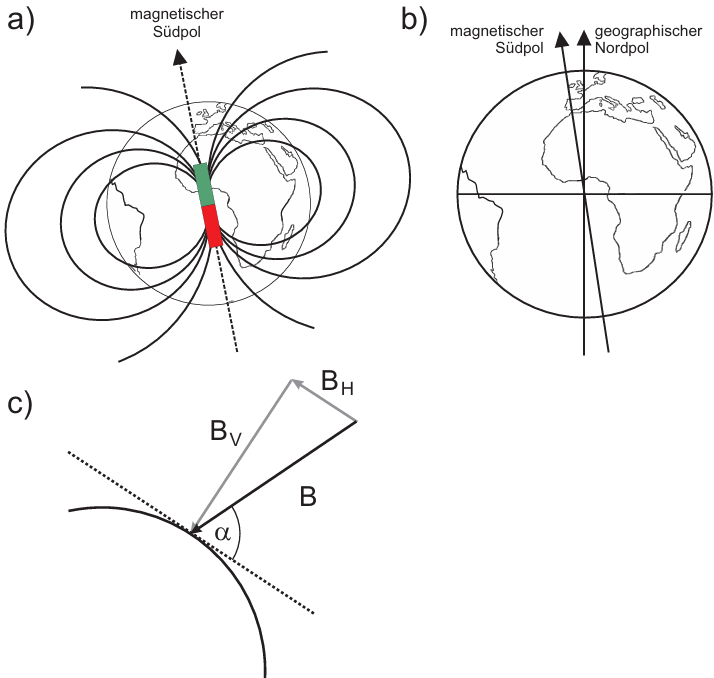
\includegraphics[width=0.5\textwidth]{files/erdmagnetfeld.png}
  \caption{Schematische Darstellungen des Erdmagnetfeldes}
  \label{fig:erdmagnetfeld}
\end{figure}
\newpage\noindent
\subsection{Versuchsdurchführung}

Der Versuch setzte sich aus vier Teilversuchen zusammen.

\textbf{Versuchsteil 1 / Vorversuch.} Der Vorversuch umfasste eine qualitative Untersuchung des Induktionseffekts. Hierzu schlossen wir eine Magnetspule direkt an das Oszilloskop an und ließen einen Magnet hindurchfallen. Der fallende Magnet erzeugte ein zeitlich veränderliches Magnetfeld, welches in der Spule eine Spannung induzierte. Diese ließ sich in Form eines Ausschlags auf dem Oszilloskop beobachten.

\textbf{Versuchsteil 2.} Im zweiten Versuchsteil befassen wir uns mit der Messung der Induktionsspannung abhängig von der Drehfrequenz der Induktionsspule (a) und dem Strom durch die felderzeugende Spule (b). 

Zur Erzeugung des Magnetfeldes verwendeten wir die Helmholtz-Spule. In deren Zentrum befand sich die kleinere Induktionsspule. Diese ließ sich an einer Aufhängung frei um eine Achse rotieren. Um eine kontinuierliche, konstante Rotation zu erzeugen war die Spule über einen Keilriemen mit einem Motor verbunden.

Für Teilaufgabe (a) betrieben wir die Helmholtz-Spule mit einem Strom von etwa $4\si{A}$ und notierten die in der Leiterschleife induzierte Spannung für einen Bereich von $3$ bis $15\si{Hz}$. Für Teilaufgabe (b) stellten wir die Leiterschleife auf eine konstante Rotation von ca. $10\si{Hz}$ und variierten für die Aufzeichnung der Induktionsspannung den Strom durch die Helmholtz-Spule in einem Bereich von $0.5$ bis $4.5\si{A}$.

\textbf{Versuchsteil 3.} Für diesen Versuchsteil legten wir an die Helmholtz-Spule eine Wechselspannung der Kreisfrequenz $\Omega$ an. Teilaufgabe (a) umfasste die Messung der Induktionsspannung für verschiedene Winkelstellungen der ruhenden Induktionsspule im Bereich von $0$ bis $360$°. In der zweiten Teilaufgabe positionierten wir die Induktionsspule in der Horizontalen in der Helmholtz-Spule und zeichneten die induzierte Spannung, sowie Spannung und Strom in der Helmholtz-Spule für verschiedene Kreisfrequenzen der angelegten Wechselspannung auf.

\textbf{Versuchsteil 4.} Im letzten Versuchsteil befassten wir uns mit dem Erdmagnetfeld. Hierzu richteten wir die Induktionsspule in Richtung des magnetischen Nordpols aus und notierten für eine Rotationsfrequenz von ca. $15\si{Hz}$ die induzierte Spannung. Dann schalteten wir die Helmholtz-Spule hinzu, um mit dieser ein Magnetfeld zu erzeugen, welches die vertikale Komponente des Erdmagnetfeldes kompensiert. Die Helmholtz-Spule mussten wir dafür auf die Seite legen. Wir notierten uns die induzierte Spannung, sowie den Strom durch die Helmholtz-Spule.